\documentclass[11pt,a4paper]{article}

\usepackage{amsmath}
\usepackage{amsfonts}
\usepackage{amssymb}
\usepackage{amsthm}

\usepackage{graphicx}

\usepackage{verbatim}

\usepackage{hyperref}


%no paragraph indent
\setlength{\parindent}{0pt}


\begin{document}

\begin{flushright}
Russ Johnson\\
Problem Set $\#1$\\
\today\\
\end{flushright}

{\bf Activity 17.4} Find, via a library or internet search, an object (building, tiling,
painting, sculpture, mosaic, fractal, rug, etc.) that has significant symmetry. Then
complete the following.\\
~\\
(a) Identify the object and the source through which you found it. Choose something other than a simple polygon; that is, find an object that is interesting to you and that possesses at least 6 symmetries, including both rotational and reflective symmetry.\\
~\\
The $K_5$ complete graph contains all of the same symmetries as a regular pentagon. It has a total of ten symmetries. The following figure is a drawing of a $K_5$ graph from wikipedia. \\
~\\
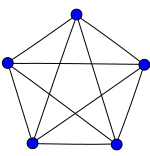
\includegraphics[scale=1]{./graphics/4-simplex_graph.pdf}
\begin{flushright}
source: \url{en.wikipedia.org/wiki/File:4-simplex_graph.svg}
\end{flushright}
~\\
b) Describe all of the symmetries possessed by your object. Choose 6 symmetries (including at least one non-trivial rotation and one non-trivial reflection), and make a copy of the picture of your object for each symmetry.
Find a convenient way to label your object so that you can use permutation notation to represent each symmetry. Then illustrate each symmetry on one of the copies of your picture.\\
~\\
The $K_5$ graph when drawn as it is from my source has reflective symmetries $r_1$, $r_2$, $r_3$, $r_4$, and $r_5$ where $r_n$'s line of symmetry is through vertex $n$ and the center of $K_5$. It also has the rotational symmetries $R_{72}$, $R_{144}$, $R_{216}$, and $R_{288}$ where $R_n$ is the rigid motion of rotation about the center of $K_5$ $n$ degrees counter-clockwise. There is also $I$ which is the rigid motion $f:O\rightarrow O$ where $f(x)=x$ for each point of the object $O$. The following is a table of symmetries for this object.\\
~\\
c) Choose 3 of the symmetries, and find all of the compositions of these three symmetries. Is each composition a symmetry of your object? Explain.\\
~\\
The following is a list of all compositions of the symmetries $r_1$, $r_2$, and $R_72$.

$
\begin{array}{rll}
r_1\circ (r_2\circ R_{72}) &= (r_1\circ r_2)\circ R_{72} &= R_{216}\\
r_1\circ (R_{72}\circ r_2) &= (r_1\circ R_{72})\circ r_2 &= R_{288}\\
r_2\circ (r_1\circ R_{72}) &=  (r_2\circ r_1)\circ R_{72} &= R_{288}\\
r_2\circ (R_{72}\circ r_1) &= (r_2\circ R_{72})\circ r_1 &= R_{144}\\
R_{72}\circ (r_1\circ r_2) &= (R_{72}\circ r_1)\circ r_2 &= R_{216}\\
R_{72}\circ (r_2\circ r_1) &= (R_{72}\circ r_2)\circ r_1 &= R_{288}\\
\end{array}
$
~\\
Each composition is a symmetry. This is due to the fact that a set of all symmetries of an object is a group under operation composition.\\
~\\
(3)\\ 
~\\
(a) Find all of the symmetries of the letter B, and create the operation table
for the set of symmetries of B.\\
~\\
There are two symmetries for the letter B, the horizontal reflection $r_H$ and $I$. The following is the operation table of these two symmetries.\\
\begin{center}
$
\begin{array}{c|c|c}
\circ & I & r_H \\\hline
I & I & r_H \\\hline
r_H & r_H & I \\
\end{array}
$\\
Symmetries of B
\end{center}
~\\
(b) Find all of the symmetries of the letter T, and create the operation table
for the set of symmetries of T.\\
~\\
There are two symmetries for the letter T, the vertical reflection, $r_v$ and $I$. The following is the operation table of these two symmetries.\\
\begin{center}
$
\begin{array}{c|c|c}
\circ & I & r_V \\\hline
I & I & r_V \\\hline
r_V & r_V & I \\
\end{array}
$\\
Symmetries of T
\end{center}
~\\
(c) Find all of the symmetries of the letter Z, and create the operation table
for the set of symmetries of Z.\\
~\\
There are two symmetries for the letter Z, a $180^\circ$ rotation, $R_{180}$ and $I$. The following is the operation table of these two symmetries.\\
\begin{center}
$
\begin{array}{c|c|c}
\circ & I & R_{180} \\\hline
I & I & R_{180} \\\hline
R_{180} & R_{180} & I \\
\end{array}
$\\
Symmetries of Z
\end{center}
~\\
(d) Compare the operation tables for B, T, and Z. Describe all of the similarities and differences you observe.\\
~\\
All of the operation tables are closed. The operation tables all have two symmetries, but $Z$ is the only letter with rotational symmetry. All three operation tables have the identity $I$ and are abelian.\\
~\\
(4) Is composition of symmetries a commutative operation? Prove your answer.\\
~\\
The composition of symmetries is not a commutative operation. A simple counter-example is that the symmetries $r_1$ and $R_{120}$ of an equilateral triangle are not commutative.\\

\[
r_1 = \left(\begin{array}{ccc}
1&2&3\\
1&3&2\\
\end{array}\right)
\]

\[
R_{120} = \left(\begin{array}{ccc}
1&2&3\\
3&1&2\\
\end{array}\right)
\]

\[
r_1\circ R_{120} = \left(\begin{array}{ccc}
1&2&3\\
2&1&3\\
\end{array}\right)
\]

\[
 R_{120}\circ r_1 = \left(\begin{array}{ccc}
1&2&3\\
3&2&1\\
\end{array}\right)
\]

From this we see that $ R_{120}\circ r_1 \neq r_1\circ R_{120}$ and so composition of symmetries is not a commutative operation for all symmetries.\\

(5) Let A, B, and C be the objects shown in Figure 17.5.\\

~\vspace{10mm}\\

(a) For each object, find all of the symmetries. Describe the symmetries in words and using the permutation notation introduced in this investigation.\\
~\\
The rectangle, A, has horizontal and vertical symmetry, a $180^\circ$ rotational symmetry, and a symmetry where we do nothing. Notationally, the symmetries are $\overline{r}_1$, $\overline{r}_2$, $R_{180}$, and $I$.\\
~\\
The pinwheel, B, has the rotational symmetries of $90^\circ$, $180^\circ$, and $270^\circ$. We can also leave it alone for a symmetry. Notationally, the symmetries are $R_{90}$,$R_{180}$, $R_{270}$, and $I$.\\
~\\
The figure-eight, C, has a $180^\circ$ rotational symmetry, a vertical, and horizontal symmetry, and itself as a symmetry. Notationally, the symmetries are $r_1$, $\overline{r}_2$, $R_{180}$, and $I$.\\
~\\
(b) Create the operation table for the set of symmetries of each object.\\
~\\
The following are the operation tables for each of the objects' symmetries.\\
~\\
\begin{center}
$
\begin{array}{c|c|c|c|c}
\circ & I & \overline{r}_1 & \overline{r}_2 & R_{180}\\\hline
I & I & \overline{r}_1 & \overline{r}_2 & R_{180}\\\hline
\overline{r}_1 & \overline{r}_1 & I & R_{180} & \overline{r}_2\\\hline
\overline{r}_2 & \overline{r}_2 & R_{180} & I & \overline{r}_1\\\hline
R_{180} & R_{180} & \overline{r}_2 &\overline{r}_1&  I\\
\end{array}
$\\
Symmetries of A Operation Table\\
~\\
$
\begin{array}{c|c|c|c|c}
\circ & I & R_{90} & R_{180} & R_{270}\\\hline
I & I & R_{90} & R_{180} & R_{270}\\\hline
R_{90} & R_{90} & R_{180} & R_{270} & I\\\hline
R_{180} & R_{180} & R_{270} & I & R_{90}\\\hline
R_{270} & R_{270} & I & R_{90} & R_{180}\\
\end{array}
$\\
~\\
Symmetries of B Operation Table\\
~\\
$
\begin{array}{c|c|c|c|c}
\circ & I & r_1 & \overline{r}_2 & R_{180}\\\hline
I & I & r_1 & \overline{r}_2 & R_{180}\\\hline
r_1 & r_1 & I & R_{180} & \overline{r}_2\\\hline
\overline{r}_2 & \overline{r}_2 & R_{180} & I & r_1\\\hline
R_{180} & R_{180} & \overline{r}_2 & r_1 & I\\
\end{array}
$\\
\end{center}

(c) Describe the similarities and differences in the operation tables you made in part (b). Your description should include not only obvious attributes like the number of elements, but also how the elements interact within a given set of symmetries.\\
~\\
Each of the operation tables are made up of four reflections and are commutative. The reason for B being commutative is that it contains only rotational symmetries. For A and C there are only two reflective symmetries.\\
~\vspace{10mm}\\
{\bf Activity 18.12.} Recall that a symmetry of an object $O$ is a bijective, distance preserving function f such that $f (O) = O$. In this activity, we will verify that the set S of symmetries of an object O forms a group under the operation of composition, called the group of symmetries of $O$.\\
~\\
(a) Let f and g be bijective, distance-preserving functions with f (O) = O
and $g(O) = O$. To show that $S$ is closed, we need to verify that $f \circ g$ is a
bijective, distance preserving function with $(f \circ g)(O) = O$.\\
~\\
(i) Prove that $|(f \circ g)(x) − (f \circ g)(y)| = |x − y|$ for all x, y in the
domain of $f \circ g$.\\
~\\
Let $S$ be the set of all symmetries of an object $O$. Let $f$ and $g$ be bijective, distance-preserving functions with $f(O)=O$ and $g(O)=O$.\\
~\\
{\bf Conjecture.} The function $f\circ g$ is a distance-preserving function.\\
\begin{proof}
We know that for all $x,y\in\mathbb{R}^2$
\begin{equation}\label{eq1}
g(x),g(y)\in\mathbb{R}^2
\end{equation}
from this fact that $g:\mathbb{R}^2\rightarrow\mathbb{R}^2$. From \eqref{eq1}  and the fact that $f$ is a distance-preserving function we also know that
\begin{equation}\label{eq2}
|f(g(x))-f(g(y))| = |g(x)-g(y)|.
\end{equation}
We also know that
\begin{equation}\label{eq3}
|g(x)-g(y)| = |x-y|
\end{equation}
from the fact that $g$ is a distance-preserving function. Using the transitive property of equality with \eqref{eq2} and \eqref{eq3} we can conclude that
\begin{align*}
|(f\circ g)(x)-(f\circ g)(y)| = |x-y|.
\end{align*}
In conclusion, we have proven that $|(f\circ g)(x)-(f\circ g)(y)| = |x-y|$ for alll $x,y\in\mathbb{R}^2$ and therefore $f\circ g$ is a distance-preserving function.
\end{proof}

(ii) Use part (a) to deduce that $f \circ g$ is an injection.\\

\begin{proof}
Let $x,y\in\mathbb{R}^2$ and
\begin{equation}\label{eq4}
(f\circ g)(x) = (f\circ g)(y)
\end{equation}
From \eqref{eq4} we can conclude that
\begin{equation}\label{eq5}
|(f\circ g)(x) - (f\circ g)(y)| = 0.
\end{equation}
We have already shown that $f\circ g$ is a distance-preserving function and so
\begin{equation}\label{eq6}
|(f\circ g)(x) - (f\circ g)(y)| = |x-y|.
\end{equation}
From \eqref{eq5}, \eqref{eq6}, and the transitive property of equality
\begin{equation}\label{eq7}
|x-y| = 0.
\end{equation}
From \eqref{eq7} and the definition of equality we can conclude
\[x=y.\]
In conclusion, we have shown that $(f\circ g)(x) = (f\circ g)(y)$ implies $x=y$ and so $f\circ g$ is an injection.
\end{proof}

(iii) Show that $(f \circ g)(O) = O$. Deduce that $f \circ g$ is a surjection.

\begin{proof}
We know that
\begin{equation}\label{iii1}
f(O) - O
\end{equation}
and
\begin{equation}\label{iii2}
g(O) = O.
\end{equation}
From \eqref{iii1} and \eqref{iii2} we can conclude that
\[f(g(O)) = O.\]
In conclusion, we have shown that $(f\circ g)(O) = O$ and therefore $f\circ g$ is surjective.

\end{proof}

(iv) Explain how parts (a)–(c) establish that S is closed under composition.\\
~\\
From parts ii and iii we have shown that $f\circ g$ is a bijective function such that $(f\circ g)(O) = O$. This is the definition of an element in $S$ and therefore $f\circ g\in S$. This establishes the fact that $S$ is closed under composition.\\
~\\
(b) Prove that composition of functions is an associative operation.

\begin{proof}
Let $h:A\rightarrow B$, $g:B\rightarrow C$, and $f:C\rightarrow D$. We will show that $(f\circ g)\circ h = f\circ (g\circ h)$. First of all, we note that $(f\circ g)\circ h:A\rightarrow D$ and $f\circ (g\circ h):A\rightarrow D$. Let $a\in A$. We know that
\begin{equation}\label{eq21}
(f\circ(g\circ h))(a)=(f\circ g)(h(a))=f(g(h(a)))
\end{equation}
and
\begin{equation}\label{22}
(f\circ(g\circ h))(a) = f((g\circ h)(a)) = f(g(h(a))).
\end{equation}
From \eqref{eq21} and \eqref{22} we can conclude that $((f\circ g)\circ h)(a) = (f\circ (g\circ h))(a)$ for all $a\in A$ and so  $(f\circ g)\circ h = f\circ (g\circ h)$.

In conclusion, we have shown that $(f\circ g)\circ h = f\circ (g\circ h)$ for the arbitrary functions $f$, $g$, and $h$. Therefore composition of functions is associative.
\end{proof}

(c) What is the identity element of S? Verify your answer.\\
~\\
The identity element of $S$ is the function $f\in S$ such that $f(x)=x$ for all x in the domain of $f$.

\begin{proof}
Let $f\in S$ be a function such that $f(x)=x$. Let $g\in S$ and $a$ be an element in the domain of $g$. We know that
\begin{equation}\label{31}
(f\circ g)(a) = f(g(a)) = g(a)
\end{equation}
and
\begin{equation}\label{32}
(g\circ f)(a) = g(f(a)) = g(a).
\end{equation}
From \eqref{31} and \eqref{32} we can conclude that the function $f$ is the identity element of $S$.
\end{proof}

(d) If f ∈ S, what is the inverse of f in S? Verify your answer. (Please note
that there is quite a bit to do to complete this problem.)\\
~\\
{\bf Conjecture.}For all $f\in S$ there must exist a left and right inverse and these two inverses are equal.
\begin{proof}
Let $f\in S$ and let $a$ be in the domain of f. We have already shown that $f$ is a bijective function. Let $g\in S$ be a function such that
\begin{equation}
(g\circ f)(x) = x
\end{equation}
\end{proof}
(e) Explain why S is a group. Is S an Abelian group? Explain.

\end{document}

Guidelines:
1. The statement of each problem must be written in its entirety, followed by the solution.

2. If you obtain an idea from someone else credit them.

3. Write in complete sentences.

4. Avoid run-ons.

5. Do not begin a sentence with a symbol.

6. As a writer, it is your job to make things clear to the reader. Do not use the words "clearly" or obviously.

7. Proofread. Use a spell-checker and be sure to re-read everything at least two times for accuracy and clarity before submitting.


Understand your audience.

Steve Schlicker

\newcommand{\c}{\circ}